\documentclass{article}
\usepackage{amsmath}
\usepackage{listings}

\usepackage{graphicx}
\graphicspath{ {./image/} }

\begin{document}

\section{CP2102}

\begin{enumerate}
    \item Connect the USB port to a desktop, a new serial port should be available.
    \item Using a serial tool(XCOM v2.0 in Windows or CuteCom in Ubuntu) to open the serial port, you will see some output. 
    \item Send "b", "y" or "r" to the device via the opened port, and the corresponding blue led, yellow led and red led will be toggled.
\end{enumerate}

\section{Speed Sensor}

\begin{enumerate}
    \item Connect external pulse signal generator to the speed sensor connectors.
    \item Open the serial port tool mentioned above, and you will read the frequencies of the pulse signal in the following format: "Speed: 0427 0427 0000 0499 0500 0499 0500 0427 0427 0854 0000 0000 0000 0499 0000 0000". Start with "Speed:", followed by 16 channels of frequency separated by a blank space. Each frequency contains 4 digits.   
    \item Note the input frequency range shall between 1~1k Hz, and will be round to an integer.
\end{enumerate}

\section{I2C Communication}
Two channels of i2c communication are used in the h750 board. One is for Communicating with PCA9685 and the other for BNO085. This test only scans the I2C addresses of those chips. 
\begin{enumerate}
    \item Open the serial port tool mentioned above. 
    \item You will see the output of the I2C addresses shown as Figure \ref{fig:i2c}
\end{enumerate}

\begin{figure}
    \centering
    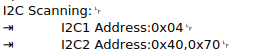
\includegraphics[totalheight=1.5cm]{i2c.png}
    \caption{I2C Message}
    \label{fig:i2c}
\end{figure}

The PCA9685 board has two I2C addresses(why?). The default I2C address of BNO085 is 0x4A.

\section{Brake}
4 channels of a timer are set to output PWM signals with the frequency of 1k Hz.
\begin{enumerate}
    \item Connect a voltage source(12V or 24V) to the connector of external high voltage. 
    \item The voltage on each channel shall be:
    \begin{enumerate}
        \item one third of the input voltage in Channel 1;
        \item two thirds of the input voltage in Channel 2;
        \item increasing from zero to the input voltage continuously in Channel 3, and
        \item decreasing from the input voltage to zero continuously in Channel 4
    \end{enumerate}    
 
\end{enumerate}

\section{ESC Signal Input}
Two input modes of ESC signal can be used.


\begin{itemize}
    \item Auto Mode: ESC and Servo pwm signals are calculated by the MPU.
    \item Manual Mode: ESC and Servo pwm signals are from an outside RC receiver.
\end{itemize} 
The input modes are switched by J?.
Test procedures:
\begin{enumerate}
    \item Open the serial port tool mentioned above. 
    \item Turn off the switch J?, the message via serial port shall contain the following strings: "Input Mode: Auto, Frequency: 50 Hz, ESC DutyCycle: 24\%, SERVO DutyCycle: 49\%". The esc output and servo output pins shall have the PWM signals output, whose frequency are 50 Hz both, and duty cycle 24 and 49, respectively.
    \item Turn on the swith J?, and connect the esc input pin and servo input pin to external PWM signals which should have the same frequency. The message should be like "Input Mode: Manual, Frequency: 63 Hz, ESC DutyCycle: 74\%, SERVO DutyCycle: 24\%", and The esc output and servo output pins shall have the same frequency and duty cycles as the input signals.
\end{enumerate}

\section{Op-Amp(Force Sensor)}
\begin{enumerate}
    \item Open the serial port tool mentioned above. 
    \item Connect the voltage selecting jumper J? to 1.2v side
    \item Adjust the potentiometer(RAD3-RAD10) to zero
    \item Connect a 100k resistor to FORCE1, and a 510k resistor to FORCE2
    \item The first element of the force in the message should be 1.81 while the second should be 0.35. 

\end{enumerate}

\end{document}